%\documentclass[12pt, a4paper]{article}
%\usepackage{tikz}
%\usepackage{cmap} 
%\usepackage[T2A]{fontenc} 
%\usepackage[utf8]{inputenc} 
%\usepackage[english,russian]{babel}
%\usepackage{amsmath}
%\usepackage[left=2cm,right=2cm,
%    top=2cm,bottom=2cm,bindingoffset=0cm]{geometry}
%\title{Алгоритмы кластеризации}
%\date{}
%\begin{document}
%\maketitle

\section*{K-means}
Алгоритм разбивает множество элементов на известное число кластеров. Основной идеей алгоритма является минимизировать среднее расстояние между каждым из объектов в кластере и его центроидом. 

\begin{itemize}

\item \( \varOmega \) = \{ \( \omega_1, \omega_2, \ldots, \omega_k \} \) -- множество кластеров.

\item \( X = \{ x_1, x_2, \ldots , x_n \} \) -- множество объектов. 

\item \( X(x_1, x_2) = \sqrt{(x_{1_1} - x_{2_1})^2 + (x_{1_2} - x_{2_2})^2 + \ldots + (x_{1_n} - x_{2_n})^2 } \) -- растояние между объектами.

\item \( \mu(\omega) = \frac{1}{|\omega|} \sum_{x \in \omega}x \) -- центроид кластера, где \( |\omega| \) -- мощность множества кластера.


\end{itemize}

\[
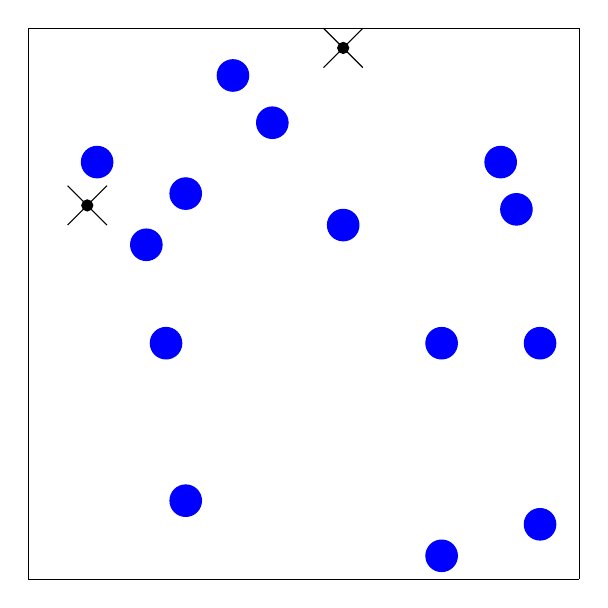
\begin{tikzpicture}
    \begin{scope}[yshift=-7.5cm, xshift=7.5cm]
        \draw (-3.5, 3.5 ) -- (3.5, 3.5);
        \draw (-3.5, -3.5) -- (3.5, -3.5);
        \draw (-3.5, -3.5) -- (-3.5, 3.5);
        \draw (3.5, 3.5) -- (3.5, -3.5);

        \draw[blue, fill=blue] (-1.5, -2.5) circle (0.2);
        \draw[blue, fill=blue] (-1.75, -0.5) circle (0.2);
        \draw[blue, fill=blue] (-1.5, 1.4) circle (0.2);
        \draw[blue, fill=blue] (-2, 0.75) circle (0.2);
        \draw[blue, fill=blue] (-2.625, 1.8) circle (0.2);
        \draw[blue, fill=blue] (1.75, -3.2) circle (0.2);
        \draw[blue, fill=blue] (3, -2.8) circle (0.2);
        \draw[blue, fill=blue] (3, -0.5) circle (0.2);
        \draw[blue, fill=blue] (1.75, -0.5) circle (0.2);
        \draw[blue, fill=blue] (2.7, 1.2) circle (0.2);
        \draw[blue, fill=blue] (2.5, 1.8) circle (0.2);
        \draw[blue, fill=blue] (0.5, 1) circle (0.2);
        \draw[blue, fill=blue] (-0.4, 2.3) circle (0.2);
        \draw[blue, fill=blue] (-0.9, 2.9) circle (0.2); 
        \draw[black] (-3, 1.5) -- (-2.5, 1);
        \draw[black] (-3, 1) -- (-2.5, 1.5);
        \draw[black] (0.25, 3) -- (0.75, 3.5);
        \draw[black] (0.25, 3.5) -- (0.75, 3);
        \filldraw[black](0.5, 3.25) circle (2pt);
        \filldraw[black] (-2.75 , 1.25) circle (2pt);
    \end{scope}
\end{tikzpicture}
\]

\begin{enumerate}

\item На первом шаге фиксируется начальное приближение. 


\[
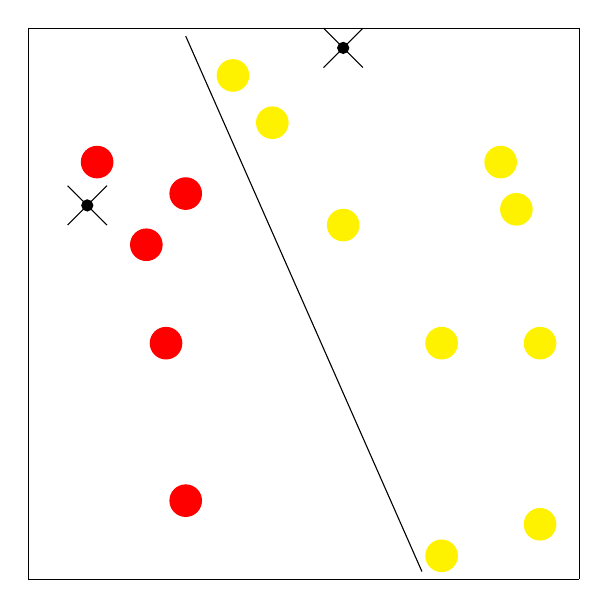
\begin{tikzpicture}
    \begin{scope}[xshift=7.5cm, yshift=7.5cm]
        \draw (-3.5, 3.5 ) -- (3.5, 3.5);
        \draw (-3.5, -3.5) -- (3.5, -3.5);
        \draw (-3.5, -3.5) -- (-3.5, 3.5);
        \draw (3.5, 3.5) -- (3.5, -3.5);

        \draw[red, fill=red] (-1.5, -2.5) circle (0.2);
        \draw[red, fill=red] (-1.75, -0.5) circle (0.2);
        \draw[red, fill=red] (-1.5, 1.4) circle (0.2);
        \draw[red, fill=red] (-2, 0.75) circle (0.2);
        \draw[red, fill=red] (-2.625, 1.8) circle (0.2);
        \draw[yellow, fill=yellow] (1.75, -3.2) circle (0.2);
        \draw[yellow, fill=yellow] (3, -2.8) circle (0.2);
        \draw[yellow, fill=yellow] (3, -0.5) circle (0.2);
        \draw[yellow, fill=yellow] (1.75, -0.5) circle (0.2);
        \draw[yellow, fill=yellow] (2.7, 1.2) circle (0.2);
        \draw[yellow, fill=yellow] (2.5, 1.8) circle (0.2);
        \draw[yellow, fill=yellow] (0.5, 1) circle (0.2);
        \draw[yellow, fill=yellow] (-0.4, 2.3) circle (0.2);
        \draw[yellow, fill=yellow] (-0.9, 2.9) circle (0.2); 
        \draw[black] (-3, 1.5) -- (-2.5, 1);
        \draw[black] (-3, 1) -- (-2.5, 1.5);
        \draw[black] (0.25, 3) -- (0.75, 3.5);
        \draw[black] (0.25, 3.5) -- (0.75, 3);
        \draw[black] (1.5, -3.4) -- (-1.5, 3.4);
        \filldraw[black](0.5, 3.25) circle (2pt);
        \filldraw[black] (-2.75 , 1.25) circle (2pt);

        
    \end{scope}
\end{tikzpicture}
\]

\item На втором шаге объекты разбиваются на кластеры, при условии минимизации расстояния от объектов до центроида. 

\[
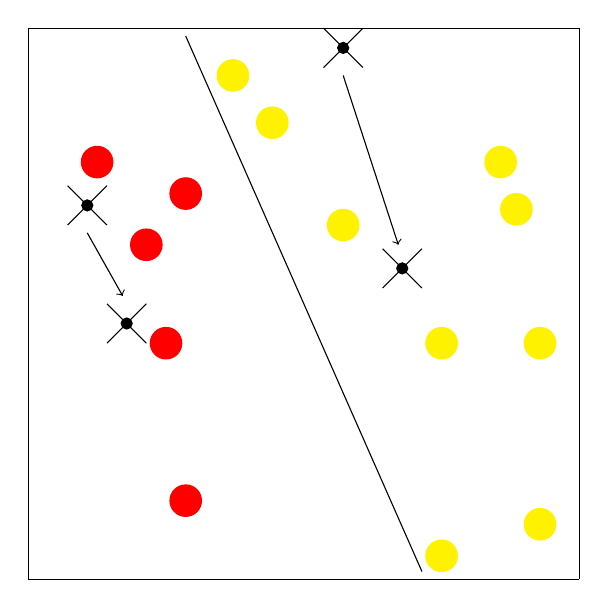
\begin{tikzpicture}
    \begin{scope}[xshift=7.5cm, yshift=7.5cm]
        \draw (-3.5, 3.5 ) -- (3.5, 3.5);
        \draw (-3.5, -3.5) -- (3.5, -3.5);
        \draw (-3.5, -3.5) -- (-3.5, 3.5);
        \draw (3.5, 3.5) -- (3.5, -3.5);

        \draw[red, fill=red] (-1.5, -2.5) circle (0.2);
        \draw[red, fill=red] (-1.75, -0.5) circle (0.2);
        \draw[red, fill=red] (-1.5, 1.4) circle (0.2);
        \draw[red, fill=red] (-2, 0.75) circle (0.2);
        \draw[red, fill=red] (-2.625, 1.8) circle (0.2);
        \draw[yellow, fill=yellow] (1.75, -3.2) circle (0.2);
        \draw[yellow, fill=yellow] (3, -2.8) circle (0.2);
        \draw[yellow, fill=yellow] (3, -0.5) circle (0.2);
        \draw[yellow, fill=yellow] (1.75, -0.5) circle (0.2);
        \draw[yellow, fill=yellow] (2.7, 1.2) circle (0.2);
        \draw[yellow, fill=yellow] (2.5, 1.8) circle (0.2);
        \draw[yellow, fill=yellow] (0.5, 1) circle (0.2);
        \draw[yellow, fill=yellow] (-0.4, 2.3) circle (0.2);
        \draw[yellow, fill=yellow] (-0.9, 2.9) circle (0.2); 
        \draw[black] (1.5, -3.4) -- (-1.5, 3.4);
        \draw[->][black] (-2.75, 0.9) -- (-2.3, 0.1);
        \draw[->][black] (0.5, 2.9) -- (1.2, 0.75);
        \draw[black] (-3, 1.5) -- (-2.5, 1);
        \draw[black] (-3, 1) -- (-2.5, 1.5);
        \draw[black] (0.25, 3) -- (0.75, 3.5);
        \draw[black] (0.25, 3.5) -- (0.75, 3);
        \filldraw[black](0.5, 3.25) circle (2pt);
        \filldraw[black] (-2.75 , 1.25) circle (2pt);
        \draw[black] (-2.5, -0.5) -- (-2, 0);
        \draw[black] (-2, -0.5) -- (-2.5, 0);
        \filldraw[black](-2.25, -0.25) circle (2pt);
        
        \draw[black] (1, 0.2) -- (1.5, 0.7);
        \draw[black] (1.5, 0.2) -- (1, 0.7);
        \filldraw[black](1.25, 0.45) circle (2pt);
        
    \end{scope}
\end{tikzpicture}
\]
\item Пересчитываются значения центроидов.

\[
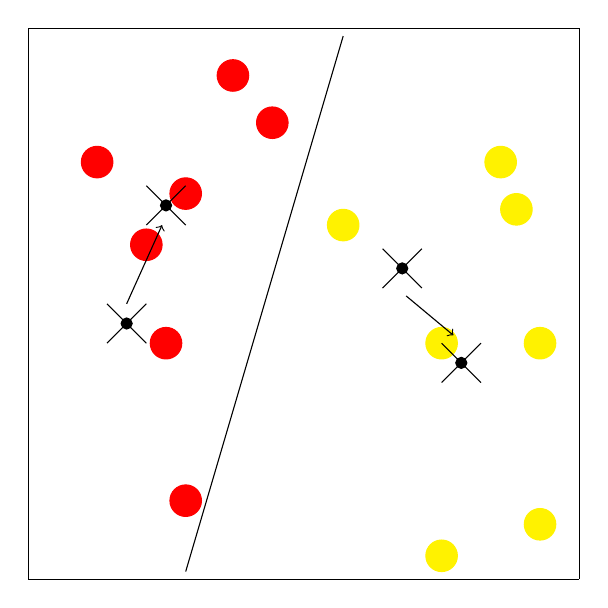
\begin{tikzpicture}
        \begin{scope}
        \draw (-3.5, 3.5 ) -- (3.5, 3.5);
        \draw (-3.5, -3.5) -- (3.5, -3.5);
        \draw (-3.5, -3.5) -- (-3.5, 3.5);
        \draw (3.5, 3.5) -- (3.5, -3.5);
    
        \draw[red, fill=red] (-1.5, -2.5) circle (0.2);
        \draw[red, fill=red] (-1.75, -0.5) circle (0.2);
        \draw[red, fill=red] (-1.5, 1.4) circle (0.2);
        \draw[red, fill=red] (-2, 0.75) circle (0.2);
        \draw[red, fill=red] (-2.625, 1.8) circle (0.2);
        \draw[yellow, fill=yellow] (1.75, -3.2) circle (0.2);
        \draw[yellow, fill=yellow] (3, -2.8) circle (0.2);
        \draw[yellow, fill=yellow] (3, -0.5) circle (0.2);
        \draw[yellow, fill=yellow] (1.75, -0.5) circle (0.2);
        \draw[yellow, fill=yellow] (2.7, 1.2) circle (0.2);
        \draw[yellow, fill=yellow] (2.5, 1.8) circle (0.2);
        \draw[yellow, fill=yellow] (0.5, 1) circle (0.2);
        \draw[red, fill=red] (-0.4, 2.3) circle (0.2);
        \draw[red, fill=red] (-0.9, 2.9) circle (0.2); 
 

        \draw[black] (0.5, 3.4) -- (-1.5, -3.4);
        \draw[->][black] (-2.25, 0) -- (-1.8, 1);
        \draw[->][black] (1.3, 0.1) -- (1.9, -0.4);
        \draw[black] (-2.5, -0.5) -- (-2, 0);
        \draw[black] (-2, -0.5) -- (-2.5, 0);
        \filldraw[black](-2.25, -0.25) circle (2pt);
        \draw[black] (1, 0.2) -- (1.5, 0.7);
        \draw[black] (1.5, 0.2) -- (1, 0.7);
        \filldraw[black](1.25, 0.45) circle (2pt);
        

        \draw[black] (-2, 1) -- (-1.5, 1.5);
        \draw[black] (-1.5, 1) -- (-2, 1.5);
        \filldraw[black](-1.75, 1.25) circle (2pt);
        
        
        \draw[black] (1.75, -1) -- (2.25, -0.5);
        \draw[black] (2.25, -1) -- (1.75, -0.5);
        \filldraw[black](2, -0.75) circle (2pt);
        
        

    \end{scope}

\end{tikzpicture}
\]

\item Алгоритм продолжается до тех пор, пока кластеры будут изменяться. 


\end{enumerate}



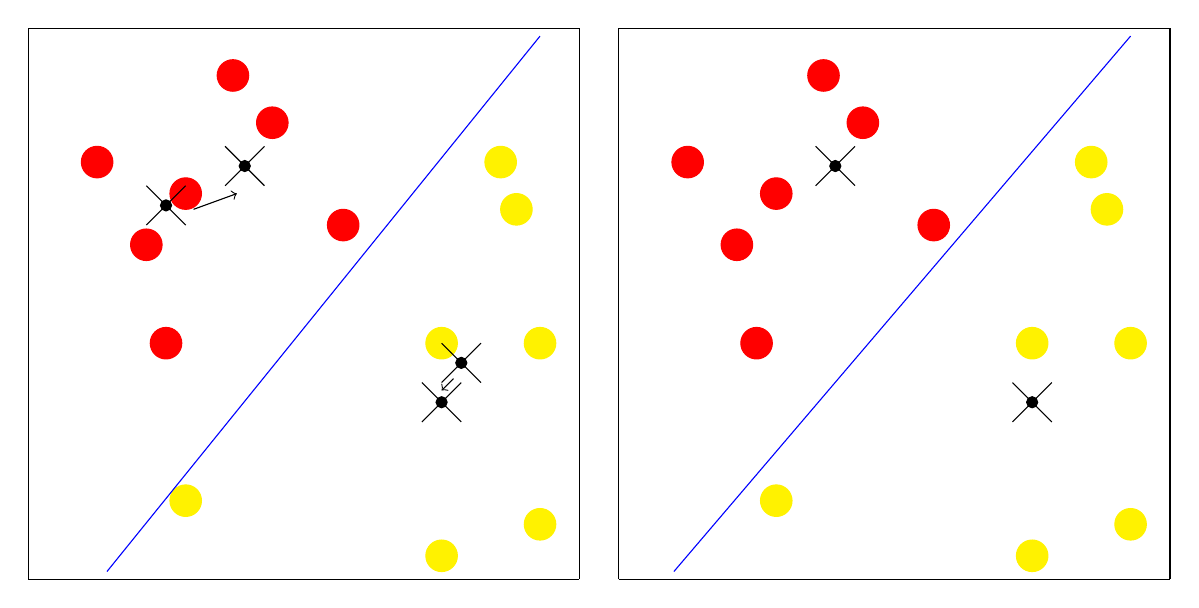
\begin{tikzpicture}
  \begin{scope}[xshift=7.5cm]
        \draw (-3.5, 3.5 ) -- (3.5, 3.5);
        \draw (-3.5, -3.5) -- (3.5, -3.5);
        \draw (-3.5, -3.5) -- (-3.5, 3.5);
        \draw (3.5, 3.5) -- (3.5, -3.5);
    
        \draw[yellow, fill=yellow] (-1.5, -2.5) circle (0.2);
        \draw[red, fill=red] (-1.75, -0.5) circle (0.2);
        \draw[red, fill=red] (-1.5, 1.4) circle (0.2);
        \draw[red, fill=red] (-2, 0.75) circle (0.2);
        \draw[red, fill=red] (-2.625, 1.8) circle (0.2);
        \draw[yellow, fill=yellow] (1.75, -3.2) circle (0.2);
        \draw[yellow, fill=yellow] (3, -2.8) circle (0.2);
        \draw[yellow, fill=yellow] (3, -0.5) circle (0.2);
        \draw[yellow, fill=yellow] (1.75, -0.5) circle (0.2);
        \draw[yellow, fill=yellow] (2.7, 1.2) circle (0.2);
        \draw[yellow, fill=yellow] (2.5, 1.8) circle (0.2);
        \draw[red, fill=red] (0.5, 1) circle (0.2);
        \draw[red, fill=red] (-0.4, 2.3) circle (0.2);
        \draw[red, fill=red] (-0.9, 2.9) circle (0.2); 

        \draw[blue] (3, 3.4) -- (-2.8, -3.4);

        \draw[black] (-1, 1.5) -- (-0.5, 2);
        \draw[black] (-0.5, 1.5) -- (-1, 2);
        \filldraw[black](-0.75, 1.75) circle (2pt);
        
        
        \draw[black] (1.5, -1.5) -- (2, -1);
        \draw[black] (2, -1.5) -- (1.5, -1);
        \filldraw[black](1.75, -1.25) circle (2pt);

        
        \end{scope}
        
 \begin{scope}
        \draw (-3.5, 3.5 ) -- (3.5, 3.5);
        \draw (-3.5, -3.5) -- (3.5, -3.5);
        \draw (-3.5, -3.5) -- (-3.5, 3.5);
        \draw (3.5, 3.5) -- (3.5, -3.5);
    
        \draw[yellow, fill=yellow] (-1.5, -2.5) circle (0.2);
        \draw[red, fill=red] (-1.75, -0.5) circle (0.2);
        \draw[red, fill=red] (-1.5, 1.4) circle (0.2);
        \draw[red, fill=red] (-2, 0.75) circle (0.2);
        \draw[red, fill=red] (-2.625, 1.8) circle (0.2);
        \draw[yellow, fill=yellow] (1.75, -3.2) circle (0.2);
        \draw[yellow, fill=yellow] (3, -2.8) circle (0.2);
        \draw[yellow, fill=yellow] (3, -0.5) circle (0.2);
        \draw[yellow, fill=yellow] (1.75, -0.5) circle (0.2);
        \draw[yellow, fill=yellow] (2.7, 1.2) circle (0.2);
        \draw[yellow, fill=yellow] (2.5, 1.8) circle (0.2);
        \draw[red, fill=red] (0.5, 1) circle (0.2);
        \draw[red, fill=red] (-0.4, 2.3) circle (0.2);
        \draw[red, fill=red] (-0.9, 2.9) circle (0.2); 

        \draw[->][black] (-1.4, 1.2) -- (-0.85, 1.4);
        \draw[->][black] (1.9, -0.95) -- (1.75, -1.1);
        \draw[blue] (3, 3.4) -- (-2.5, -3.4);
                
        \draw[black] (-1, 1.5) -- (-0.5, 2);
        \draw[black] (-0.5, 1.5) -- (-1, 2);
        \filldraw[black](-0.75, 1.75) circle (2pt);
        
        
        \draw[black] (1.5, -1.5) -- (2, -1);
        \draw[black] (2, -1.5) -- (1.5, -1);
        \filldraw[black](1.75, -1.25) circle (2pt);
        
        \draw[black] (-2, 1) -- (-1.5, 1.5);
        \draw[black] (-1.5, 1) -- (-2, 1.5);
        \filldraw[black](-1.75, 1.25) circle (2pt);
        
        
        \draw[black] (1.75, -1) -- (2.25, -0.5);
        \draw[black] (2.25, -1) -- (1.75, -0.5);
        \filldraw[black](2, -0.75) circle (2pt);
    \end{scope}

  
\end{tikzpicture}





%\end{document}